\graphicspath{{./1-Proyecto/capitulo2/}}

\chapter{Archimate}{
    \section{Introducción}
    En el contexto de la Arquitectura Empresarial, contar con un lenguaje de modelado estandarizado resulta esencial para representar de manera clara y coherente los diferentes dominios organizacionales. En este sentido, Archimate surge como una solución práctica y ampliamente adoptada que permite modelar, describir, analizar y comunicar arquitecturas complejas de forma estructurada.

    ArchiMate es un lenguaje de modelado abierto, desarrollado y respaldado por The Open Group, que proporciona una notación visual unificada para representar las relaciones entre procesos de negocio, aplicaciones y tecnología. Su objetivo es facilitar la comprensión de la arquitectura empresarial tanto para los equipos técnicos como para los diferentes grupos de interés de una organización, permitiendo una visión integral y coherente del estado actual y futuro de la empresa.

    Gracias a su enfoque estructurado, Archimate permite visualizar cómo los cambios en un área afectan a otras, promoviendo la alineación estratégica entre el negocio y las tecnologías de la información. Asimismo, ofrece una base sólida para el análisis de impacto, la toma de decisiones y la gestión de transformaciones organizacionales.

    Este capítulo explora las bases conceptuales de Archimate, sus principales características, y su papel como lenguaje complementario dentro del desarrollo de la arquitectura empresarial con TOGAF.
	\section{¿Qué es Archimate?}
    \textbf{ArchiMate es un lenguaje de modelado de arquitectura empresarial} abierto e independiente para respaldar la descripción, el análisis y la visualización de la arquitectura dentro y entre dominios comerciales de manera inequívoca.\\\
    ArchiMate ofrece un lenguaje común para describir la construcción y operación de procesos comerciales, estructuras organizativas, flujos de información, sistemas de TI e infraestructura técnica. Esta información ayuda a las partes interesadas a diseñar, evaluar y comunicar las consecuencias de las decisiones y los cambios dentro y entre estos dominios comerciales. \cite{Archimate_definition}
	\section{Características}	
	ArchiMate es un  estándar abierto  mantenido y actualizado por The Open Group. Se tienen en cuenta los últimos desarrollos e ideas en arquitectura empresarial y el marco ArchiMate se mejora continuamente. Algunas de las características que posee Archimate son:
    \begin{itemize}
        \item ArchiMate garantiza la coherencia en todos los modelos de arquitectura, por lo que es un lenguaje ágil y sencillo. 
        \item Contiene suficientes conceptos para modelar la arquitectura empresarial y no incluye todos los conceptos posibles para no salirse de sus propios límites. Como resultado, la arquitectura empresarial se puede comunicar de manera clara y coherente en todos los dominios de su negocio. 
        \item Su estructura uniforme hace que sea fácil de aprender y aplicar.
        \item ArchiMate permite realizar un modelado de alto nivel dentro de un dominio, es también bases para el análisis de identificación de procesos, actores, entre otros elementos involucrados en una arquitectura empresarial, este lenguaje se ofrece así como un complemento que ofrece metodologías que permiten desarrollar una arquitectura empresarial.
        \item ArchiMate ofrece una forma de generalización de comunicación a nivel empresarial, lo que potencializa la velocidad con la cual se puede conocer un proceso o elemento que pertenece a una arquitectura empresarial.
    \end{itemize}
    
    %---------------------- CAPA DE RELACIONES ------------------------%
    \section{Capas}
    
    %--------------------------------------------CAPA DE APLICACIÓN ------------------------------------------------------%
    
    \subsection{Capa de aplicación}
    
    Los elementos de la capa de aplicación se utilizan normalmente para modelar la arquitectura de la aplicación que describe la \textbf{estructura, el comportamiento y la interacción de las aplicaciones de la empresa}.
    
    La tabla \ref{tab:Tabla de la capa de aplicación}  ofrece una descripción general de los elementos de la capa de aplicación, con sus definiciones.\cite{archimate} 
    
    
    \begin{longtable}{|p{0.15\linewidth}|p{0.45\linewidth}|p{0.2\linewidth} p{0.2\linewidth}|}
    	\caption{Tabla de la capa de aplicación}
    	\\
    	\hline
    	\rowcolor[HTML]{AFC5F6} 
    	\textbf{Elemento} & \textbf{Descripción} & \multicolumn{2}{c|}{\textbf{Notación}} \\
    	\hline
    	\endhead
    	\hline
    	\multicolumn{4}{r}{\textit{Continúa en la siguiente página}} \\
    	\endfoot
    	\hline
    	\endlastfoot
    	\label{tab:Tabla de la capa de aplicación}
    	%Contenido 1 &
    	%\lipsum[1] &
    	%Datos A1
    	%& Datos B1
    	%\\
    	%\hline
    	
    	
    	
    	Componente de Aplicación 
    	&
    	Representa una parte modular, reemplazable y desplegable de un sistema de software que encapsula su comportamiento y datos. 
    	&
    	\begin{center}
    		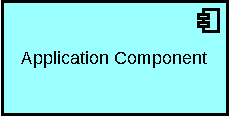
\includegraphics[width=1\linewidth]{imgs/aplication_component.pdf}
    	\end{center} 
    	&
    	\begin{center}
    		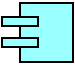
\includegraphics[width=0.5\linewidth]{imgs/component.pdf}
    	\end{center}
    	\\ \hline
    	
    	
    	
    	Colaboración de Aplicación 
    	&
    	Indica una unidad de comportamiento colectivo que agrupa componentes de aplicación para ofrecer una funcionalidad empresarial conjunta. 
    	&
    	\begin{center}
    		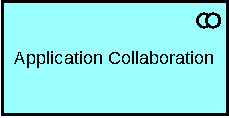
\includegraphics[width=1\linewidth]{imgs/Aplication_collaboration.pdf}
    	\end{center} &
    	\begin{center}
    		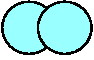
\includegraphics[width=0.7\linewidth]{imgs/collaboration.pdf}
    	\end{center}
    	\\ \hline
    	
    	
    	
    	Interfaz de Aplicación 
    	&
    	Representa un punto de acceso en el que los servicios de la aplicación se ponen a disposición de un usuario, otro componente de la aplicación o un nodo. 
    	&
    	\begin{center}
    		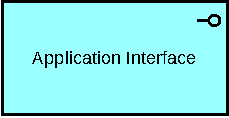
\includegraphics[width=1\linewidth]{imgs/Aplication_interface.pdf}
    	\end{center} &
    	\begin{center}
    		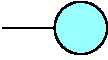
\includegraphics[width=0.7\linewidth]{imgs/interfaz.pdf}
    	\end{center}
    	\\ \hline
    	
    	
    	
    	Función de Aplicación 
    	&
    	Representa el comportamiento automatizado que puede realizar un componente de la aplicación. 
    	&
    	\begin{center}
    		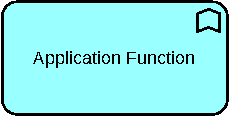
\includegraphics[width=1\linewidth]{imgs/Aplication_function.pdf}
    	\end{center} &
    	\begin{center}
    		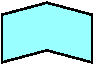
\includegraphics[width=0.7\linewidth]{imgs/function.pdf}
    	\end{center}
    	\\ \hline
    	
    	Interacción de Aplicación 
    	&
    	Representa una unidad de comportamiento colectivo de la aplicación realizada por (una colaboración de) dos o más componentes de la aplicación. 
    	&
    	\begin{center}
    		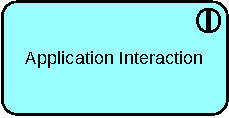
\includegraphics[width=1\linewidth]{imgs/Aplication_interaction.pdf}
    	\end{center} &
    	\begin{center}
    		
\includegraphics[width=0.7\linewidth]{imgs/interaction.pdf}
    	\end{center}
    	\\ \hline
    	
    	Proceso de Aplicación 
    	&
    	Representa una secuencia de comportamientos de la aplicación que logra un resultado específico. 
    	&
    	\begin{center}
    		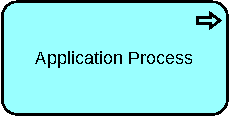
\includegraphics[width=1\linewidth]{imgs/aplication_process.pdf}
    	\end{center} &
    	\begin{center}
    		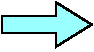
\includegraphics[width=0.7\linewidth]{imgs/process.pdf}
    	\end{center}
    	\\ \hline
    	
    	Evento de Aplicación 
    	&
    	Representa un cambio de estado de la aplicación. 
    	&
    	\begin{center}
    		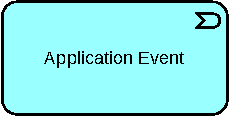
\includegraphics[width=1\linewidth]{imgs/Aplication_event.pdf}
    	\end{center} &
    	\begin{center}
    		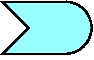
\includegraphics[width=0.7\linewidth]{imgs/event.pdf}
    	\end{center}
    	\\ \hline
    	
    	
    	Servicio de Aplicación 
    	&
    	Representa un comportamiento de aplicación expuesto definido explícitamente. 
    	&
    	\begin{center}
    		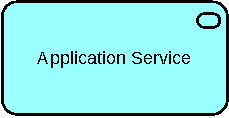
\includegraphics[width=1\linewidth]{imgs/Aplication_service.pdf}
    	\end{center} &
    	\begin{center}
    		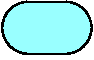
\includegraphics[width=0.7\linewidth]{imgs/service.pdf}
    	\end{center}
    	\\ \hline
    	
    	
    	Objeto de Datos 
    	&
    	Representa datos estructurados para su tratamiento automatizado. 
    	&
    	\begin{center}
    		\includegraphics[width=1\linewidth]{imgs/aplication_dataObject.pdf}
    	\end{center} &
    	\begin{center}
    		\includegraphics[width=0.7\linewidth]{imgs/Data_object.pdf}
    	\end{center}
    	\\ \hline
    \end{longtable}
}